\documentclass[12pt, a4paper]{article}

\usepackage[czech]{babel}
\usepackage{lmodern}
\usepackage[utf8]{inputenc}
\usepackage[T1]{fontenc}
\usepackage[pdftex]{graphicx}
\usepackage{amsmath, amssymb}
\usepackage[hidelinks,unicode]{hyperref}
\usepackage{float}
\usepackage{listings}
\usepackage{tikz}
\usepackage{xcolor}
\usepackage{tabularx}
\usepackage[final]{pdfpages}
\usepackage{syntax}
\usepackage{caption}
\usepackage{subcaption}
\usepackage{amsfonts}


\definecolor{mauve}{rgb}{0.58,0,0.82}
\usetikzlibrary{shapes,positioning,matrix,arrows}

\newcommand{\img}[1]{(viz obr. \ref{#1})}

\definecolor{pblue}{rgb}{0.13,0.13,1}
\definecolor{pgreen}{rgb}{0,0.5,0}
\definecolor{pred}{rgb}{0.9,0,0}
\definecolor{pgrey}{rgb}{0.46,0.45,0.48}


\lstdefinestyle{flex}{
    frame=tb,
    aboveskip=3mm,
    belowskip=3mm,
    showstringspaces=false,
    columns=flexible,
    basicstyle={\small\ttfamily},
    numbers=none,
    numberstyle=\tiny\color{black},
    keywordstyle=\color{black},
    commentstyle=\color{black},
    stringstyle=\color{black},
    breaklines=true,
    breakatwhitespace=true,
    tabsize=3
}

\lstset{
    frame=tb,
    language=Python,
    aboveskip=3mm,
    belowskip=3mm,
    showstringspaces=false,
    columns=flexible,
    basicstyle={\small\ttfamily},
    numbers=none,
    numberstyle=\tiny\color{gray},
    keywordstyle=\color{blue},
    commentstyle=\color{pgreen},
    stringstyle=\color{mauve},
    breaklines=true,
    breakatwhitespace=true,
    tabsize=3
}


\let\oldsection\section
\renewcommand\section{\clearpage\oldsection}

\begin{document}
	% this has to be placed here, after document has been created
	% \counterwithout{lstlisting}{chapter}
	\renewcommand{\lstlistingname}{Ukázka kódu}
	\renewcommand{\lstlistlistingname}{Seznam ukázek kódu}
    \begin{titlepage}

        \centering

        \vspace*{\baselineskip}
        \begin{figure}[H]
        \centering
        
\includegraphics[width=7cm]{img/fav-logo.jpg}
        \end{figure}

        \vspace*{1\baselineskip}

        \vspace{0.75\baselineskip}

        \vspace{0.5\baselineskip}
        {Domácí úkol z předmětu KIV/VSS}

        {\LARGE\sc Generátory náhodných čísel\\}
        {\sc s Poissonovo rozdělením\\}

        \vspace{4\baselineskip}

        \vspace{0.5\baselineskip}

        {\sc\Large Stanislav Král \\}
        \vspace{0.5\baselineskip}
        {A20N0091P}

        \vfill

        {\sc Západočeská univerzita v Plzni\\
        Fakulta aplikovaných věd}

    \end{titlepage}

    % TOC
    \tableofcontents
    \pagebreak

\section{Zadání}
S využitím knihovní funkce pro generování pseudonáhodných čísel vytvořte generátor \textbf{Poissonovo} rozdělení jako funkci v jazyce Java, C, C++, Pascal/Delphi (kdy parametry rozdělení jsou zároveň parametry funkce generátoru) s využitím vhodné metody (inverzní transformace, kompoziční metoda, vylučovací metoda, atd.).

\section{Poissonovo rozdělení}
    Jedná se o rozdělení pravděpodobnosti, které popisuje diskrétní náhodnou veličinu vyjadřující počet výyskytů jevů v určitém intervalu, pokud jevy nastávají nezávisle na sobě a dílčí intervaly mezi jevy mají exponenciální rozdělení s parametrem 1.
Toto rozdělení se používá k aproximaci binomického rozdělení pro velký počet pokusů a malou pravděpodobnost výskytu sledovaného jevu v jednom pokusu.

    Jediným parametrem tohoto rozdělení je $\lambda$, který představuje střední hodnotu a rozptyl Poissonovo rozdělení. Tento parametr musí být z intervalu $(0, \infty)$.

     Diskrétní náhodná veličina $X$ se řídí Poissonovo rozdělením, pokud s použitím parametru $\lambda > 0$ má funkce hustoty pravděpodobnosti rozdělení následující tvar:
    \begin{displaymath}
       \!f(k; \lambda)= \Pr(X{=}k)= \frac{\lambda^k e^{-\lambda}}{k!}
    \end{displaymath}

    \begin{figure}[!ht]
        \centering
        \begin{minipage}{.5\textwidth}
            \centering
            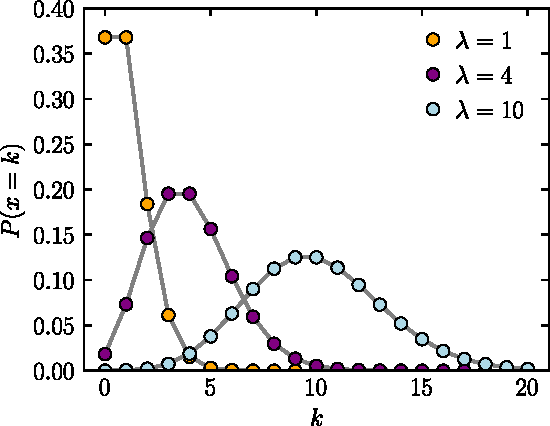
\includegraphics[width=.95\linewidth]{pdf/pmf.pdf}
            \captionof{figure}{Graf hustoty ppstní. funkce}
            \label{fig:test1}
        \end{minipage}%
        \begin{minipage}{.5\textwidth}
            \centering
            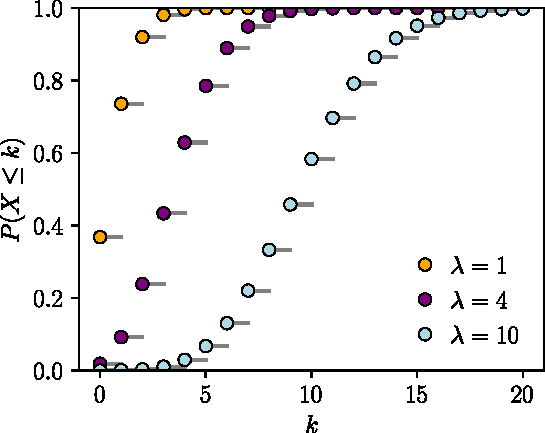
\includegraphics[width=.95\linewidth]{pdf/cdf.pdf}
            \captionof{figure}{Graf funkce rozdělení}
            \label{fig:test2}
        \end{minipage}
    \end{figure}

    Praktické využití Poissonova rozdělení lze pozorovat například při modelování vytížení telefonní ústředny, modelování rizika výskytu zemětřesení nebo modelování počtu fotonů dopadajících na teleskop\footnote{Rasch, Georg (1963), \hyperlink{http://www.rasch.org/memo1963.pdf}{"The Poisson Process as a Model for a Diversity of Behavioural Phenomena"} (PDF), 17th International Congress of Psychology, 2, Washington, DC, USA, August 20th – 26th, 1963: American Psychological Association}.

    \newpage
    \subsection{Střední hodnota} \label{expectedvaluesec}
    K odvození střední hodnoty Poissonova rozdělení s parametrem $\lambda$ lze použít následující postup:


    \begin{equation}
        \label{expectedvalue}
        \begin{split}
        \mathbb{E}(X) &= \sum_{x \mathop \in X} x\,Pr(X = x) \\
        \mathbb{E}(X) & = \sum_{x=0}^{\infty}x\frac{\lambda^{x}}{x!}e^{-\lambda} \\
        & = \lambda\,e^{-\lambda}\sum_{x=0}^{\infty} \frac{\lambda^{x-1}}{(x-1)!} \\
        & = \lambda\,e^{-\lambda}e^{\lambda} \\
        & = \lambda
        \end{split}
    \end{equation}

    \subsection{Rozptyl} \label{variancesec}
    K odvození rozptylu Poissonova rozdělení s parametrem $\lambda$ lze použít následující postup\footnote{dle \url{https://proofwiki.org/wiki/Variance_of_Poisson_Distribution/Proof_1}}:

    \begin{equation}
        \label{variance}
        \begin{split}
            var\,(X) & = \mathbb{E} (X^2) - (\mathbb{E} (X))^2 \\
            \mathbb{E} (X^2) &= \sum_{x \mathop \in \Omega_{X}} x^2 \, Pr(X = x) \\
            \mathbb{E} (X^2) &= \sum_{k \mathop \ge 0} {k^2 \dfrac 1 {k!} \lambda^k e^{-\lambda} } \\
            & = \lambda\, e^{-\lambda} \sum_{k \mathop \ge 1} {k \dfrac 1 {(k - 1)!} \lambda^{k - 1} } \\
            & = \lambda\, e^{-\lambda} ( \sum_{k \mathop \ge 1} {(k - 1) \dfrac 1 {(k - 1)!} \lambda^{k - 1} } + \sum_{k \mathop \ge 1} {\frac 1 {(k - 1)!} \lambda^{k - 1} }  ) \\
            & = \lambda\, e^{-\lambda} ( \lambda \sum_{k \mathop \ge 2} {\dfrac 1 {(k - 2)!} \lambda^{k - 2} } + \sum_{k \mathop \ge 1} {\dfrac 1 {(k - 1)!} \lambda^{k - 1} } ) \\
            & = \lambda\, e^{-\lambda} ( \lambda \sum_{i \mathop \ge 0} {\dfrac 1 {i!} \lambda^i} + \sum_{j \mathop \ge 0} {\dfrac 1 {j!} \lambda^j} ) \\
            & = \lambda\, e^{-\lambda} ( \lambda e^\lambda + e^\lambda) \\
            & = \lambda\, e^{-\lambda} ( \lambda e^\lambda + e^\lambda) \\
            & = \lambda^2 + \lambda \\
            var\,(X) & = \lambda^{2} + \lambda - \lambda^{2} = \lambda \\
        \end{split}
    \end{equation}


    \section{Implementace generátoru náhodných čísel}

    V rámci tohoto úkolu byl naimplementován generátor náhodných čísel s Poissonovo rozdělením v jazyce Python (verze 3).
    Vytvořený program se skládá ze čtyř Python skriptů:
    \begin{itemize}
        \item \texttt{distribution\_tester.py} -- načtení vstupních parametrů a ověření vlastností generátoru náhodných čísel (výpočet střední hodnoty, rozptylu a sestavení histogramu),
        kdy jako první parametr přijímá velikost vzorku, který se použije pro ověření výstupu generátoru, a druhý parametr
        použije jako parametr $\lambda$ Poissonova rozdělení.
        \item \texttt{histogram.py} -- definice metod pro vykreslení histogramu
        \item \texttt{poisson.py} -- implementace generátoru náhodných čísel řídících se Poissonovo rozdělením
        \item \texttt{stat_utils.py} -- definice metod pro výpočet střední hodnoty, rozptylu a směrodatné odchylky z vytvořené řady náhodných čísel
    \end{itemize}

    Pro jednodušší spuštění byl ještě vytvořen bash skript \texttt{poisson.sh}, který předává vstupní parametry skriptu
    \texttt{distribution\_tester.py}.

    \subsection{Třída \texttt{PoissonDistribution}}

    Tato třída poskytuje rozhraní pro generování náhodných čísel, výpočet hodnoty funkce hustoty pravděpodobnosti a distribuční
    funkce Poissonova rozdělení, kdy výpočet druhé zmíněné funkce je realizován pomocí sčítání hodnot funkce hustoty
    pravděpodobnosti rozdělení.

    Aby bylo možné generovat náhodná čísla řídící se Poissonovo rozdělením s využitím knihovní funkce pro generování
    pseudonáhodných čísel, tak je třeba transformovat rovnoměrné rozdělení na intervalu $(0, 1)$ (poskytované knihovní funkcí
    \texttt{random.uniform(0, 1)}) na Poissonovo rozdělení s vybraným parametrem $\lambda$.
    Jelikož je Poissonovo rozdělení diskrétní, tak pro transformaci není příliš vhodné použít vylučovací metodu, avšak
    použít lze také, jelikož je známa funkce hustoty pravděpodobnosti Poissonova rozdělení.
    U transformace ale narážíme na problém, že výpočet distribuční funkce Poissonova rozdělení není jednoduchý, a tak je
    třeba najít jiný způsob, jak požadované hodnoty funkce zjistit.

    Pro jednoduchost byla ve vytvořeném programu použita metoda, která počítá hodnoty distribuční funkce pomocí
    sčítání hodnot funkce hustoty (čímž provádí numerický výpočet určitého integrálu funkce hustoty).

    \begin{lstlisting}
        def cdf(self, n):
            # calculate the CDF by summing PMF  values
            return sum([self.pmf(k) for k in range(0, n + 1)])
    \end{lstlisting}

    \noindent Z optimalizačních důvodů se výsledky výpočtů ukládají do paměti.

    Inverzní distribuční funkce je aproximována pomocí tabulky, do které se předpočítávají výsledky distribuční funkce.

    Při inicializaci instance třídy \texttt{PoissonDistribution} je předpočítáváno minimálně $2.5\, \lambda$ hodnot nebo tolik
    hodnot, kolik je třeba, aby rozdíl dvou po sobě jdoucích hodnot distribuční funkce byl menší než požadovaný rozdíl $\epsilon$.

   \begin{lstlisting}
def initialize(self, e):
    # initialize the generator by generating initial values INV CDF values
    diff = 1
    last_cdf = 0
    n = 0
    # compute CDF values till the lambda * 2.5 values generated or till the difference
    # before the current cdf and the previous one is smaller than a certain constant
    while n < self.rate * 2.5 or diff > e:
        cdf = self.cdf(n)
        diff = abs(last_cdf - cdf)
        last_cdf = cdf
        n += 1
   \end{lstlisting}

    Inicializací se zajistí naplnění tabulky pro výpočet hodnot inverzní distribuční funkce. Konstanty $2.5\, \lambda$ a
    rozdíl $\epsilon$ určují přesnost aproximace.

    Výhoda této metody oproti použití vylučovací metody je ta, že doba potřebná k výpočtu požadované hodnoty distribuční funkce je
    deterministická, nikoliv náhodná.

    Generování náhodných čísel je pak realizováno následující jednoduchou metodou, kde do inverzní distrubuční funkce vstupují
    čísla z generátoru řídícího se uniformním rozdělením $X \sim (0, 1)$:

    \begin{lstlisting}
def rand(self):
    return self.cdf_inv(random.uniform(0, 1))
    \end{lstlisting}

    Za zmínku stojí Knuthův algoritmus\footnote{Knuth, Donald Ervin (1997), Seminumerical Algorithms, \hyperlink{https://en.wikipedia.org/wiki/The\_Art\_of\_Computer\_Programming}{The Art of Computer Programming}, 2 (3rd ed.), Addison Wesley, ISBN 978-0-201-89684-8}, který sice negeneruje náhodná čísla v deterministickém čase, avšak jeho implementace
    je velmi jednoduchá. Ve třídě \texttt{PoissonDistribution} je tento algoritmus implementován pomocí metody \texttt{rand\_knuth}.
    Pro ověření tohoto generátoru pomocí skriptu \texttt{distribution_tester.py} stačí pouze přejmenovat tuto metodu na \texttt{rand}.

    \pagebreak

    \begin{lstlisting}
def rand_knuth(self):
    # alternative random number generator following Poisson distribution implementation
    # using Knuth's algorithm
    l = math.exp(-self.rate)
    p = 1.0
    k = 0
    while True:
        k += 1
        p *= random.uniform(0, 1)
        if p <= l:
            break
    return k - 1
    \end{lstlisting}

    \subsection{Výpočet střední hodnoty}
    Metoda \texttt{expected\_value} pro výpočet střední hodnoty se nachází ve skriptu \texttt{stat\_utils.py}, kdy jako parametr očekává tabulku,
    která představuje histogram (klíče tabulky představují hodnotu a hodnoty tabulky představují četnosti hodnot dle klíče).
    Výpočet je implementací obecného vzorce pro výpočet střední hodnoty ukázaný v \ref{expectedvaluesec}.

    \begin{lstlisting}
def expected_value(histogram):
    total = sum(histogram.values())
    return sum([value * frequency / total for value, frequency in histogram.items()])
    \end{lstlisting}
    
    \subsection{Výpočet rozptylu}
    Metoda \texttt{variance} pro výpočet rozptylu se nachází ve skriptu \texttt{stat\_utils.py}, kdy jako parametr očekává tabulku,
    která představuje histogram (struktura tabulky stejná jako u předchozí metody).
    Během výpočtu volá pro zjištění střední hodnoty $\mathbb{E}(X)$ metodu \texttt{expected\_value}.
    Výpočet je implementací obecného vzorce pro výpočet rozptylu ukázaný v \ref{variancesec}.

    \begin{lstlisting}
def variance(histogram):
    ev = expected_value(histogram)
    total = sum(histogram.values())
    return sum([((value - ev) ** 2) * (frequency / total) for value, frequency in histogram.items()])
    \end{lstlisting}

    \subsection{Výpočet směrodatné odchylky}
    Metoda \texttt{standard\_deviation} pro výpočet směrodatné odhylky se nachází ve skriptu \texttt{stat\_utils.py}, kdy jako parametr očekává tabulku,
    která představuje histogram (struktura stejná jako u předchozí metody).

    Výpočet je implementací obecného vzorce pro výpočet směrodatné odchylky.
    
    \section{Výsledky implementovaného generátoru}

    Následující text obsahuje výstup programu\footnote{kombinace se použijí, pokud je testovací skript spuštěn bez povinných parametrů} během testování generátoru náhodných čísel pro následující kombinace parametrů:

    \begin{enumerate}
        \item Velikost testovacího vzorku: \texttt{10000}, $\lambda=5$
        \item Velikost testovacího vzorku: \texttt{100000}, $\lambda=9$
    \end{enumerate}

    \begin{lstlisting}[basicstyle=\tiny]
Default test case #1 rate=5, n=10000
------------------------------------
E_teorie=5
D_teorie=5
E_vypocet=5.0063
D_vypocet=5.03586031

HISTOGRAM
0.0000 :***
1.0000 :**********
2.0000 :************************
3.0000 :**************************************
4.0000 :*************************************************
5.0000 :***************************************************
6.0000 :*****************************************
7.0000 :******************************
8.0000 :******************
9.0000 :**********
10.0000:******
11.0000:***
12.0000:**
13.0000:*
14.0000:*
15.0000:*

Default test case #2 rate=9, n=100000
-------------------------------------
E_teorie=9
D_teorie=9
E_vypocet=8.99288
D_vypocet=8.9687293056

HISTOGRAM
0.0000 :*
1.0000 :*
2.0000 :**
3.0000 :******
4.0000 :*************
5.0000 :************************
6.0000 :***********************************
7.0000 :*********************************************
8.0000 :***************************************************
9.0000 :**************************************************
10.0000:*********************************************
11.0000:*************************************
12.0000:****************************
13.0000:********************
14.0000:*************
15.0000:********
16.0000:*****
17.0000:***
18.0000:*
19.0000:*
20.0000:*
21.0000:*
22.0000:*
23.0000:*
24.0000:*
25.0000:*
    \end{lstlisting}

    Z výsledků testování lze pozorovat, že dochází k očekávané odchylce od teoretické střední hodnoty a rozptylu, která je způsobena
    aproximací inverzní distribuční funkce, výstupem pseudonáhodného generátoru \texttt{random.uniform} a hlavně tím,
    že velikost testovacího vzorku se limitně neblíží k nekonečnu. Mezi další faktory, které ovlivňují velikost odchylky,
    určitě patří i skutečnost, že procesory mají pouze omezenou přesnost při počítání s desetinnými čísly.

    Generování náhodných čísel je díky zvolené implementaci deterministické, a tak by bylo možné ho použít např. pro
    systémy, kde je tato vlastnost požadovaná.

    Odchylky od očekávaných hodnot nejsou příliš velké a i při pohledu na zobrazený histogram lze konstatovat, že
    výstup generátoru je možné modelovat Poissonovo rozdělením, čímž je splněno zadání domácího úkolu.

    \end{document}
